\documentclass{vldb}
\usepackage{graphicx}
\usepackage{caption}
\usepackage{float}
\usepackage[table,xcdraw]{xcolor}
\usepackage{hyperref}

\begin{document}

% ****************** TITLE ****************************************

\title{Assignment 2 - DB2}

% ****************** AUTHORS **************************************

\numberofauthors{2} 

\author{
% 1st. author
\alignauthor Daniel Brand
% 2nd. author
\alignauthor Andreas Kostecka
}


\maketitle

\section{Concurrency control mechanisms}

Describe briefly the concurrency control mechanisms supported by your DBMS.\\

For concurrency control and prevention from uncontrolled data access the DB2 database manager offers locking for bufferpools, tables, data partitions,
blocks and rows. A lock associates a resource of the database manager from an application. This application is called the lock owner.  A lock controls the 
concurrent access of the same resource from other applications held by the lock owner.\\


The database manager uses locking at a row or table level but always attempts to acquire row-level locks.
The decision of the locking level is based on several factors:
\begin{itemize}
\item Active isolation level 
\item Database access method (index scan or table scan)
\item Specified \textbf{LOCKSIZE} attribute for a certain table
(see section~\ref{sec:task3})
\item Available space for locks depending on the \textbf{LOCKLIST} size and/or \textbf{MAXLOCKS} parameter
\begin{itemize}
\item LOCKLIST: The amount of memory, defined in 4KiB pages, reserved to manage locks for all
connected applications
\item MAXLOCKS: Maximum percentage of the entire lock list a single application can hold
\end{itemize}
\end{itemize}

The duration a lock is alive depends on the isolation level:
\begin{itemize}
\item Uncommitted-Read-Search: If row data isn't altered, row locking is deactivated
\item Cursor-Stability-Search: Row locks are active as long as de cursor is positioned at the corresponding row. 
In this case it is possible that no locks are active
\item Read-Stability-Search: Row locks for rows that fits the search criterion are valid as long as the transaction is active
\item Repeatable-Read-Search: All row locks are valid as long as the transaction is active
\end{itemize}

\section{Locking modes}

What lock modes are supported by your DBMS (shared, exclusive, others)?\\

DB2 supports the following lock modes:
\begin{enumerate}
\item Intent None (IN)
\begin{itemize}
\item Applicable-Objects: Tablespaces, tables, blocks, data partitions
\item Description: Lock owner can read locked data in the object, also uncommitted data, but isn't allowed to alter this data. Lock owner doesn't acquire row-level locks. 
Other concurrent running applications can read and alter data.
\end{itemize}
\item Intent Share (IS)
\begin{itemize}
\item Applicable-Objects: Tablespaces, tables, blocks, data partitions
\item Description: Lock owner can read locked data in the table, but isn't allowed to alter this data. Other applications can read and alter data in the table.
\end{itemize}
\item Intent Exclusive (IX)
\begin{itemize}
\item Applicable-Objects: Tablespaces, tables, blocks, data partitions
\item Description: Lock owner and concurrent running applications can read and alter data. Other concurrent running applications can read and update the table.
\end{itemize}
\item Scan Share (NS)
\begin{itemize}
\item Applicable-Objects: Rows
\item Description: Lock owner and concurrent running applications can read the locked rows, but aren't allowed to alter these rows. When the isolation level of the
application is Cursor-Stability (CS) or Read-Stability (RS) this lock mode is used instead of a normal Share (S) lock. 
\end{itemize}
\item Next Key Weak Exclusive (NW)
\begin{itemize}
\item Applicable-Objects: Tablespaces, tables, blocks, data partitions
\item Description: If a row is inserted into an index the next row acquires a NW lock. This occurs only when the next row is locked by an Repeatable-Read-Search.
The lock owner can read the row but not alter.
\end{itemize}
\item Share (S)
\begin{itemize}
\item Applicable-Objects: Rows, tables, blocks, data partitions
\item Description: Lock owner and concurrent running applications can read the locked data but not alter.
\end{itemize}
\item Share with Intent Exclusive (SIX)
\begin{itemize}
\item Applicable-Objects: Tables, blocks, data partitions
\item Description: Lock owner can read and alter data. Other concurrent running applications can only read the table.
\end{itemize}
\item Update (U)
\begin{itemize}
\item Applicable-Objects: Rows, tables, blocks, data partitions
\item Description: Lock owner can alter data. Other transactions (units of work) can read the locked data in the object but aren't allowed to alter the data.
\end{itemize}
\item Exclusive (X)
\begin{itemize}
\item Applicable-Objects: Rows, tables, blocks, data partitions, bufferpools
\item Description: Lock owner can read and alter data in the locked object. Only applications running with the isolation level Uncommitted-Read (UR)
can access the locked object.
\end{itemize}
\item Super Exclusive (Z)
\begin{itemize}
\item Applicable-Objects: Tablespaces, tables, blocks, data partitions
\item Description: Lock owner can alter, drop the table or create, drop an index. This lock is automatically granted whenever a transaction uses one of these
operations. No other concurrent running application can read or alter this table.
\end{itemize}
\end{enumerate}

\begin{table}[H]
\small
\begin{tabular}{|
>{\columncolor[HTML]{C0C0C0}}c |c|c|c|c|c|c|c|c|c|c|}
\hline
{\color[HTML]{333333} \textbf{}} & \cellcolor[HTML]{C0C0C0}{\color[HTML]{333333} IN} & \cellcolor[HTML]{C0C0C0}{\color[HTML]{333333} IS} & \cellcolor[HTML]{C0C0C0}{\color[HTML]{333333} NS} & \cellcolor[HTML]{C0C0C0}{\color[HTML]{333333} S} & \cellcolor[HTML]{C0C0C0}{\color[HTML]{333333} IX} & \cellcolor[HTML]{C0C0C0}{\color[HTML]{333333} SIX} & \cellcolor[HTML]{C0C0C0}{\color[HTML]{333333} U} & \cellcolor[HTML]{C0C0C0}{\color[HTML]{333333} X} & \cellcolor[HTML]{C0C0C0}{\color[HTML]{333333} Z} & \cellcolor[HTML]{C0C0C0}{\color[HTML]{333333} NW} \\ \hline
IN & Y & Y & Y & Y & Y & Y & Y & Y & X & Y \\ \hline
IS & Y & Y & Y & Y & Y & Y & Y & X & X & X \\ \hline
NS & Y & Y & Y & Y & X & X & Y & X & X & Y \\ \hline
S & Y & Y & Y & Y & X & X & Y & X & X & X \\ \hline
IX & Y & Y & X & X & Y & X & X & X & X & X \\ \hline
SIX & Y & Y & X & X & X & X & X & X & X & X \\ \hline
U & Y & Y & Y & Y & X & X & X & X & X & X \\ \hline
X & Y & X & X & X & X & X & X & X & X & X \\ \hline
Z & X & X & X & X & X & X & X & X & X & X \\ \hline
NW & Y & X & Y & X & X & X & X & X & X & X \\ \hline
\end{tabular}
\caption{Lock mode compatibility matrix (Y - compatible, X - not compatible)}
\end{table}

\section{Resource locking}
\label{sec:task3}
Which resource types can be locked in your DBMS (schema, tables, rows, others)?

Show on simple examples how (if possible) to explicitly lock resources (for example, tables and tuples)?\\

DB2 supports locking for the following types:
\begin{itemize}
\item Bufferpools
\item  Tables
\item Data-Partitions (partitioned tables)
\item Blocks
\item Rows
\end{itemize}

With the command \textbf{ALTER TABLE} a global lock granularity can be set:
\begin{itemize}
\item Rows
\begin{verbatim}
ALTER TABLE TABLE_NAME LOCKSIZE ROW
\end{verbatim}
\item Blockinserts
\begin{verbatim}
ALTER TABLE TABLE_NAME LOCKSIZE BLOCKINSERT
\end{verbatim}
\item Tables
\begin{verbatim}
ALTER TABLE TABLE_NAME LOCKSIZE TABLE
\end{verbatim}
\end{itemize}

With the command \textbf{LOCK TABLE} an application can lock a table on application level:
\begin{itemize}
\item Share-Mode:
\begin{verbatim}
LOCK TABLE TABLE_NAME IN SHARE MODE
\end{verbatim}
Prevents concurrent application processes from executing any except read-only operations on the table.
\item Exclusive-Mode:
\begin{verbatim}
LOCK TABLE TABLE_NAME IN EXCLUSIVE MODE
\end{verbatim}
Prevents concurrent application processes from executing any operations on the table. EXCLUSIVE MODE does not prevent concurrent application 
processes running at isolation level Uncommitted Read (UR) from executing read-only operations on the table.
\end{itemize}

A bufferpool lock is granted as soon as a bufferpool is created, altered or deleted. Bufferpools have always exclusive locks.

\section{Booking experiment}

\subsection{Remarks} For IBM's database system DB2 the \textit{ROW LOCKING} can be set by the SQL - statement \textbf{ALTER TABLE LOCKSIZE ROW}. Since DB2 is based on the SQL92 standard, no boolean data type is supported (not for columns at least), so we simulated them by using an Integer with the values 1 and 0. The simulation utility was written in Java. The test was done on a 6-core processor with a local DB2 installation on a SSD.

\subsection{Results}
\subsubsection{Execution times and booking tries}
In figure \ref{img:lineplot1} we can see the almost identical execution times, if it were not for the single transaction, serialized test. The execution times for this test were significantly larger than for any other test. The times for other tests vary within a few hundred milliseconds.
\begin{figure}[H]
	\centering
	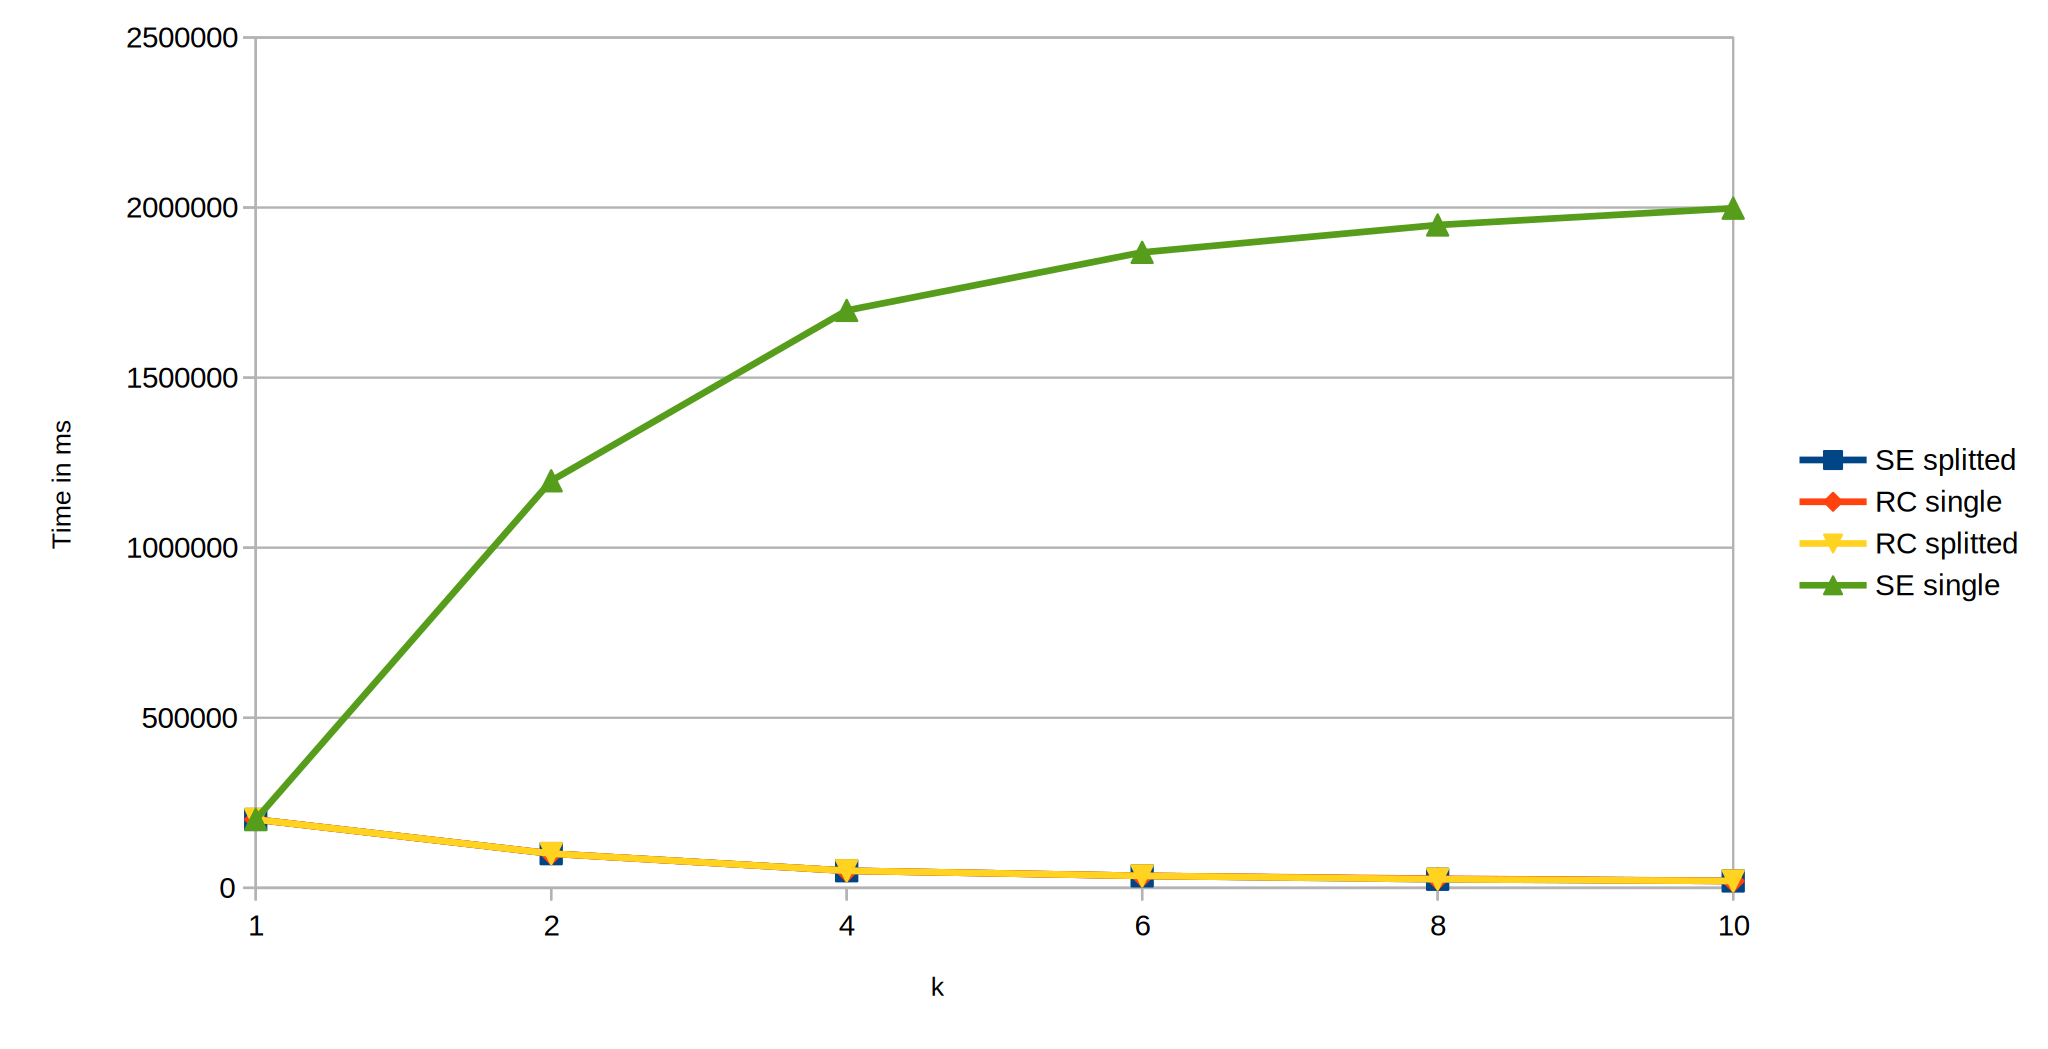
\includegraphics[width=0.43\textwidth]{results-jdbc-isolevels/lineplot.png}
	\caption{Line plot for all tests}
	\label{img:lineplot1}
\end{figure}
To see the curve for the tests better, we omitted the single transaction, serialize test for figure \ref{img:lineplot2};
\begin{figure}[H]
	\centering
	\includegraphics[width=0.43\textwidth]{results-jdbc-isolevels/lineplot-without-singleserliaze.png}
	\caption{Line plot without single transaction, serialize test}
	\label{img:lineplot2}
\end{figure}
The tables \ref{tab:rcbookings1} \ref{tab:sebookings1} show the average, minimal and maximal booking tries for the isolation levels read committed and serializable respectively.
\begin{table}[H]
	\small \centering
	\begin{tabular}{|
			>{\columncolor[HTML]{C0C0C0}}c |c|c|c|c|c|c|}
		\hline
		{\color[HTML]{333333} \textbf{Threads:}} & \cellcolor[HTML]{C0C0C0}{\color[HTML]{333333} 1} & \cellcolor[HTML]{C0C0C0}{\color[HTML]{333333} 2} & \cellcolor[HTML]{C0C0C0}{\color[HTML]{333333} 4} & \cellcolor[HTML]{C0C0C0}{\color[HTML]{333333} 6} & \cellcolor[HTML]{C0C0C0}{\color[HTML]{333333} 8} & \cellcolor[HTML]{C0C0C0}{\color[HTML]{333333} 10} \\ \hline
		\multicolumn{7}{|c|}{Read committed single}\\ \hline
		min: & 1 & 1 & 1 & 1 & 1 & 1 \\ \hline
		max: & 1 & 1 & 1 & 1 & 1 & 1\\ \hline
		avg: & 1 & 1 & 1 & 1 & 1 & 1\\ \hline
		\multicolumn{7}{|c|}{Read committed splitted}\\ \hline
		min: & 1 & 1 & 1 & 1 & 1 & 1 \\ \hline
		max: & 1 & 1 & 1 & 1 & 1 & 1\\ \hline
		avg: & 1 & 1 & 1 & 1 & 1 & 1\\ \hline
	\end{tabular}
	\caption{Booking tries for isolation level \textbf{Read committed}}
	\label{tab:rcbookings1}
\end{table}
\begin{table}[H]
	\small \centering
	\begin{tabular}{|
			>{\columncolor[HTML]{C0C0C0}}c |c|c|c|c|c|c|}
		\hline
		{\color[HTML]{333333} \textbf{Threads:}} & \cellcolor[HTML]{C0C0C0}{\color[HTML]{333333} 1} & \cellcolor[HTML]{C0C0C0}{\color[HTML]{333333} 2} & \cellcolor[HTML]{C0C0C0}{\color[HTML]{333333} 4} & \cellcolor[HTML]{C0C0C0}{\color[HTML]{333333} 6} & \cellcolor[HTML]{C0C0C0}{\color[HTML]{333333} 8} & \cellcolor[HTML]{C0C0C0}{\color[HTML]{333333} 10} \\ \hline
		\multicolumn{7}{|c|}{Serializable single}\\ \hline
		min: & 1 & 1 & 1 & 1 & 1 & 1 \\ \hline
		max: & 1 & 101 & 151 & 168 & 176 & 181\\ \hline
		avg: & 1 & 1.5 & 2.5 & 3.525 & 4.5 & 5.5\\ \hline
		\multicolumn{7}{|c|}{Serializable splitted}\\ \hline
		min: & 1 & 1 & 1 & 1 & 1 & 1 \\ \hline
		max: & 1 & 1 & 1 & 1 & 1 & 1\\ \hline
		avg: & 1 & 1 & 1 & 1 & 1 & 1\\ \hline
	\end{tabular}
	\caption{Booking tries for isolation level \textbf{Serializable}}
	\label{tab:sebookings1}
\end{table}
The numbers of (re-)tries for booking a seat seem to correlate with the observed execution times. The only way for DB2 and our program to trigger a retry was setting the isolation level to serializable and using a single transaction. We are unsure whether our implementation has issues or this behavior simply follows through the nature of DB2 and the properties of this exercise.
\subsubsection{Resulting tables}
We decided to look at that aspect too. Since at the end of a test each row should have value \textit{false} for column \textit{availability}, we looked at the remaining \textit{true} entries. Table \ref{tab:fail1} shows the row counts for tables with an availability field set to \textit{true}.
\begin{table}[H]
	\small \centering
	\begin{tabular}{|
			>{\columncolor[HTML]{C0C0C0}}c |c|c|c|c|c|c|}
		\hline
		{\color[HTML]{333333} \textbf{Threads:}} & \cellcolor[HTML]{C0C0C0}{\color[HTML]{333333} 1} & \cellcolor[HTML]{C0C0C0}{\color[HTML]{333333} 2} & \cellcolor[HTML]{C0C0C0}{\color[HTML]{333333} 4} & \cellcolor[HTML]{C0C0C0}{\color[HTML]{333333} 6} & \cellcolor[HTML]{C0C0C0}{\color[HTML]{333333} 8} & \cellcolor[HTML]{C0C0C0}{\color[HTML]{333333} 10} \\ \hline
		\multicolumn{7}{|c|}{Read committed}\\ \hline
		Single: & 0 & 4 & 8 & 10 & 15 & 24 \\ \hline
		Splitted: & 0 & 3 & 5 & 9 & 21 & 15\\ \hline
		\multicolumn{7}{|c|}{Serializable}\\ \hline
		Single: & 0 & 0 & 0 & 0 & 0 & 0 \\ \hline
		Splitted: & 0 & 1 & 7 & 9 & 14 & 15\\ \hline
	\end{tabular}
	\caption{Absolute failure rates}
	\label{tab:fail1}
\end{table}
Looking at the results for a single thread, a zero mark was expected, since only one thread accesses the database at a time. With an increasing thread count, the failures, i.e. a seat doubly set to \textit{not available}, rise too, with the worst value 24 for isolation level read committed on 10 threads. The only way to guarantee a correct booking for our implementation and using DB2 was using a single transaction with isolation level serializable.

\subsection{Results with PreparedStatements}
For the previous results we used the class \textit{java.sql.Statement} throughout the program. Because the execution times were that bad, we tried replacing the \textit{java.sql.PreparedStatement} class for all taxing commands, i.e. \textit{SELECT}, \textit{UPDATE} and \textit{INSERT}. The overall times did indeed decrease by a small margin, but 1 second at most. The failure rates seem to be better though, for isolation level serializable at least.

\begin{table}[H]
	\small \centering
	\begin{tabular}{|
			>{\columncolor[HTML]{C0C0C0}}c |c|c|c|c|c|c|}
		\hline
		{\color[HTML]{333333} \textbf{Threads:}} & \cellcolor[HTML]{C0C0C0}{\color[HTML]{333333} 1} & \cellcolor[HTML]{C0C0C0}{\color[HTML]{333333} 2} & \cellcolor[HTML]{C0C0C0}{\color[HTML]{333333} 4} & \cellcolor[HTML]{C0C0C0}{\color[HTML]{333333} 6} & \cellcolor[HTML]{C0C0C0}{\color[HTML]{333333} 8} & \cellcolor[HTML]{C0C0C0}{\color[HTML]{333333} 10} \\ \hline
		\multicolumn{7}{|c|}{Read committed}\\ \hline
		Single: & 0 & 3 & 5 & 15 & 16 & 20 \\ \hline
		Splitted: & 0 & 1 & 9 & 11 & 21 & 20\\ \hline
		\multicolumn{7}{|c|}{Serializable}\\ \hline
		Single: & 0 & 0 & 0 & 0 & 0 & 0 \\ \hline
		Splitted: & 0 & 1 & 3 & 5 & 12 & 16\\ \hline
	\end{tabular}
	\caption{Absolute failure rates}
	\label{tab:fail2}
\end{table}
\section{Viewing locks [optional]}
DB2 ships with a utility called \textbf{db2pd}, which is intended for error handling or correction. With that tool you can display a massive amount of information like memory usage, accessing applications and locks currently held.

To show the currently held locks:
\begin{verbatim}
db2pd -db DATABASE\_NAME -locks
\end{verbatim}
An example output of that would be:
\begin{verbatim}
Database Member 0 -- Database FSR -- Active -- 
Up 0 days 00:26:33 -- Date 2015-11-08 ...

Locks:
Address            TranHdl    Lockname          ...
0x00007F45D791A600 11         0700000002000000
0x00007F45D7918880 12         0700000002000000
0x00007F45D791A100 12         0700000001000000
0x00007F45D7918B00 11         0700000001000000
0x00007F45D791B500 12         5359534C564C3031
0x00007F45D7911B00 11         5359534C564C3031
0x00007F45D7913280 12         0200040000000000
0x00007F45D7917E80 11         0200040000000000  ...
\end{verbatim}

These are locks held during execution of our program in exercise 4 for this assignment. To show further information on those locks the option \textbf{showlocks} can be added. By using 
\begin{verbatim}
db2 "SELECT SUBSTR(TABSCHEMA,1,8) AS TABSCHEMA,\
SUBSTR(TABNAME,1,15) AS TABNAME, LOCK_OBJECT_TYPE,\
LOCK_MODE, LOCK_MODE_REQUESTED, AGENT_ID_HOLDING_LK\
FROM SYSIBMADM.LOCKWAITS WHERE AGENT_ID = 000"
\end{verbatim}
the currently held locks of a process with the AGENT\_ID 000 are emitted.

\end{document}
